\documentclass{article}
\usepackage{amsmath}
\usepackage{listings}
\usepackage{algorithm2e}
\usepackage{enumitem}
\usepackage{graphicx}
\graphicspath{./}
\begin{document}
\title {CS 260 Homework 4}
\author{Semanti Basu}
\maketitle


\section*{Question 1}
\begin{enumerate}
\item The nodes which are leaves are: D,M,N,F,J,K,L
\item Node A is root
\item Parent of node c is A
\item Nodes F,G,H are children of C
\item Ancestors of E are B and A
\item Descendants of E are I,M and N
\item Right sibling of D=E, Right sibling of E=none
\item J and F are to the left of G and K,H,L are to the right of G.
\item Depth of C is 1
\item Height of C is 2
\end{enumerate}

\section*{Question 2}
There are 6 different paths of length three
\begin{itemize}
\item $A->C->H->L$
\item $A->C->G->K$
\item $A->C->G->J$
\item $A->B->E->I$
\item $B->E->I->M$
\item $B->E->I->N$
\end{itemize}

\section*{Question 3}
\subsection*{n is to the left of m}
\begin{itemize}
\item pr(n) $<$ pr(m) = True
\item in(n) $<$ in(m) = True
\item po(n) $<$ po(m) = True
\end{itemize}

\subsection*{n is to the right of m}
\begin{itemize}
\item pr(n) $<$ pr(m) = False
\item in(n) $<$ in(m) = False
\item po(n) $<$ po(m) = True
\end{itemize}

\subsection*{n is a proper ancestor of m}
\begin{itemize}
\item pr(n) $<$ pr(m) = True
\item in(n) $<$ in(m) = True
\item po(n) $<$ po(m) = False
\end{itemize}

\subsection*{n is a proper descendant of m}
\begin{itemize}
\item pr(n) $<$ pr(m) = False
\item in(n) $<$ in(m) = True
\item po(n) $<$ po(m) = True
\end{itemize}

\section*{Question 4}
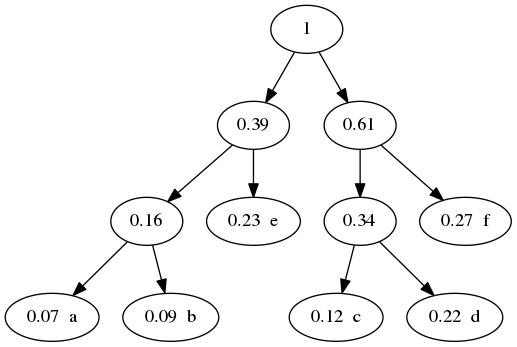
\includegraphics[scale=0.5]{bTree.png}




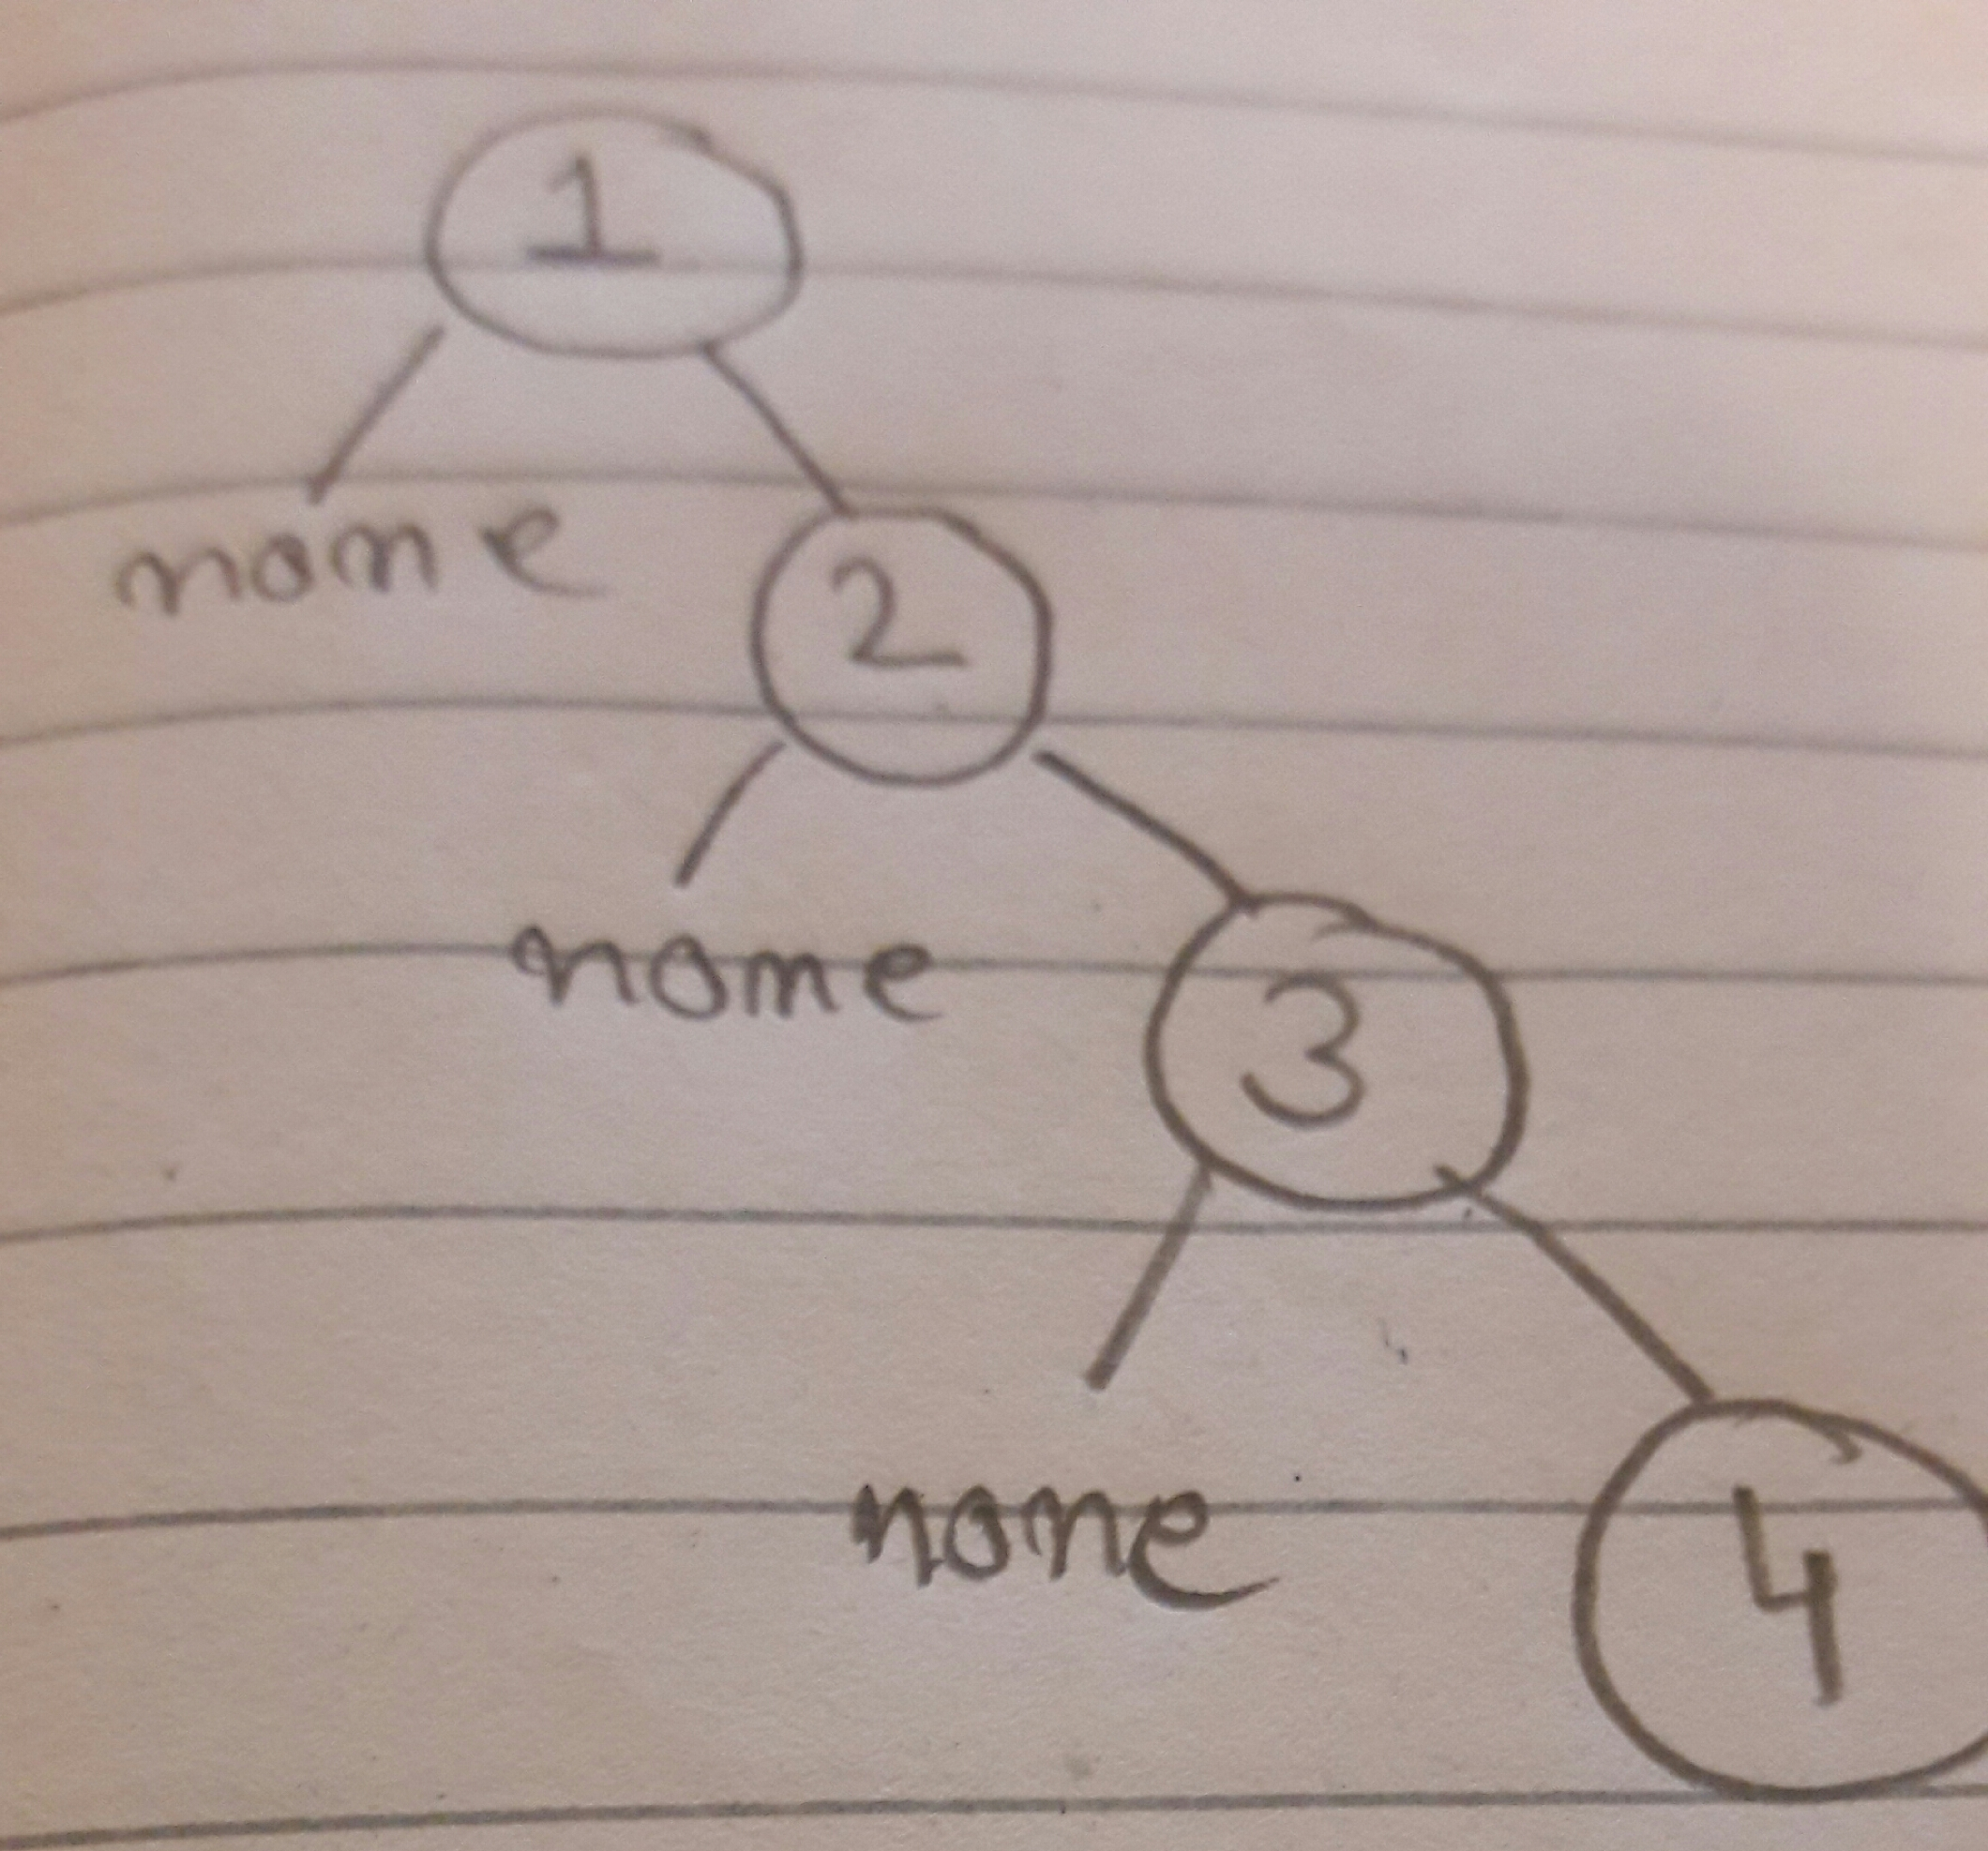
\includegraphics[scale=0.05]{1.jpg}

\subsection*{Huffman codes}
0 is put on left branches and 1 on the right branches to generate code.




\begin{tabular}{c c}
\hline\hline
letter & code\\
a & 000\\
b & 001\\
c & 100\\
d & 101\\
e & 01\\
f & 11\\
\end{tabular}


\subsection*{average length}
Average length=$3*0.07+0.09*3+0.12*3+0.22*3+0.23*2+0.27*2$=2.5

\section*{Question 5}

Maximum height = n-1

Since there are n nodes, the maximum height of the tree occurs when each node has exactly one child. The height of the tree is the number of edges 
between root to leaf. When each node except leaf has exactly one child in a binary tree, then the number of edges comes up to n-1.

Minimum height=$\log_2 n$

To minimise the height of the tree, we can make sure that each level of the binary tree is completely filled before moving to the next level.
This can be done by making sure that each node in the current level has exactly two children before moving on to the next level. If we have a binary tree with n nodes such that each node 
has 2 children, then the height of the tree is $\log_2 n$ which is also the minimum height an n-node binary tree can attain.


\section*{Question 6}

Maximum height = n-1

Since there are n nodes, the maximum height of the tree occurs when each node has exactly one child. The height of the tree is the number of edges
between root to leaf. When each node except leaf has exactly one child in the tree, then the number of edges comes up to n-1.

Minimum height=floor($\log_b n$)

To minimise the height of the tree, we can make sure that each level of the tree is completely filled before moving to the next level.
This can be done by making sure that each node in the current level has exactly b children before moving on to the next level. If we have a tree with n nodes such that each node
has b children, then the height of the tree is $\log_b n$ which is also the minimum height an n-node tree can attain.So, if b=2, the tree will be a binary tree. In that case, for 0-1 nodes,
the height will be 0.For 2- 3 nodes the height will 1. For 4 - 7 nodes the height will be 2 etc.For b-ary tree, the minimum height will be, $\log_b n$.



\end{document}
